\section {Design and Implementation\\}

\subsection{Reactor Model\\}
The PushUp server runs atop of the Twisted framework\cite{Twisted}, an 
event driven framework that implements the ``reactor" style event loop.

The reactor patterns is an event processing pattern for handling concurrent
service requests. It demultiplexes these requests to associated event
handlers(implemented as the callback). The event handler performs
the actual read or write synchronously.

In our project the reactor manages event loops (one Reactor 
can start several event loops) and runs in a single thread. The
Twisted's event loop has well encapsulated the OSes' underlying 
event notification mechanism (for example, kqueue() in FreeBSD 
and epoll() in Linux).
During execution, the event loop manages the details regarding to
event handler registrations, the activations of event handlers, etc.

The advantage of the reactor patter is the complete separation of the 
application specific code from the reactor implementation. That is to
say, the application components can be easily divided into reusable 
modulars. Also, running the reactor in a single threads significantly
reduce the concurrency controls since no other threads will contend 
the system resource instantaneously.

Figure \ref{fig:mainloop} demonstrates the how the execution switches
between the event loops and user code. Figure \ref{fig:eventloop_flow} 
further illustrates the detailed work flow with sequence diagram.

As we can see from these figures, one of the caveats of in 
event-driven development is that all the event handlers should 
be carefully designed in order to make sure its execution time 
will not take a long time; otherwise the whole system will 
be blocked.

\begin{figure}[htb!]
    \centering%
    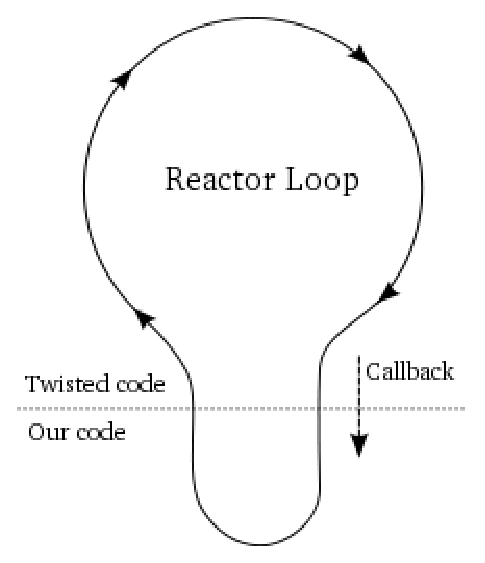
\includegraphics[scale=0.75]{figures/mainloop.eps}
    \caption{Work flow of Twisted Reactor Model}
    \label{fig:mainloop}
\end{figure}
\begin{figure}[htb!]
    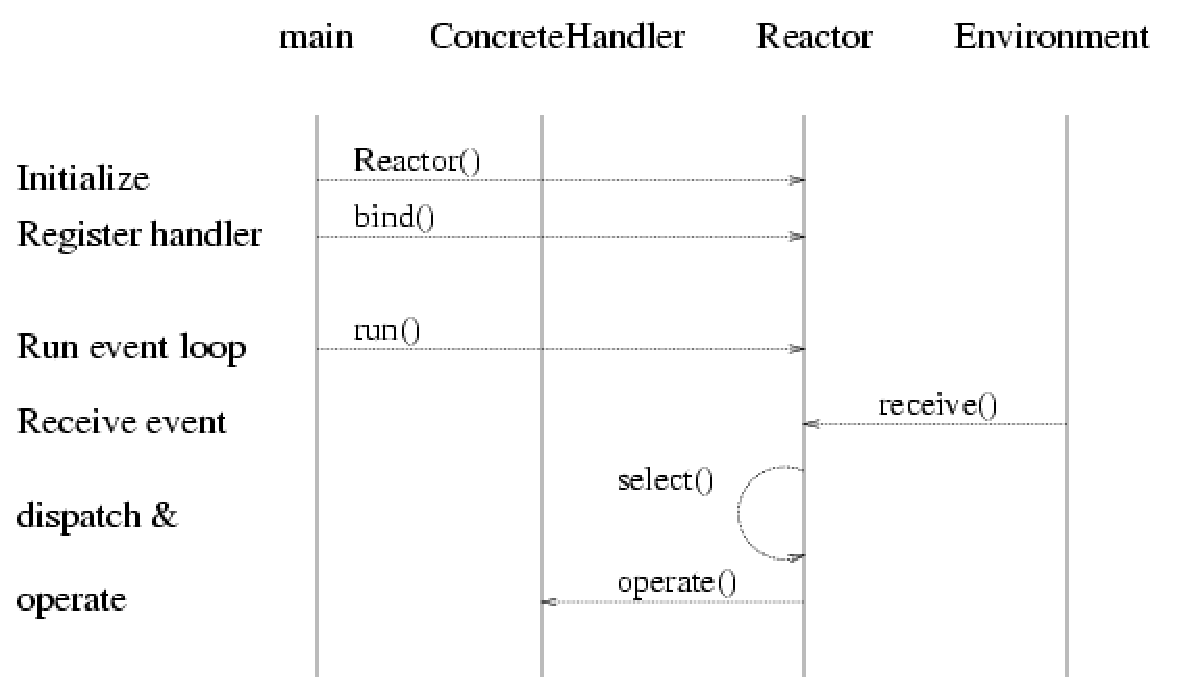
\includegraphics[scale=0.45]{figures/eventloop_flow.eps}
    \caption{The Sequence Diagram of the Event Loop}
    \label{fig:eventloop_flow}
\end{figure}


\subsection{Channels\\}

A ``channel" represents message stream of a certain type. For example, a
channel may be used to represent the feed of a specific user's tweets in
twitter, or the articles of a blog. The channel is the building block of 
PushUp's message queue.

The channel has two major responsibilities: manages the subscription and
incoming messages in this channel.

A complete subscription includes the following information:

\begin{itemize}
    \item {\bf Timeout(required)}: the channel will keep the subscription 
        connection open only for a certain timespan. If nothing happens 
        during this period, the
        subscription request will be terminated and removed from the active 
        subscription list by the channel.
    \item {\bf Time Range(optional)}: the client may specify the ``start time"
        and ``end time" of its interested messages. Since the channel 
        caches all the incoming messages for a certain time(we will explain this later), 
        proper time range should be specified otherwise the client will 
        always receive all the available messages in the channel (this is
        because if the time range is not specified, by default the channel
        will set the start time to be $0$ and the end time to be 
        $max\_int$).

        Owing to the stateless nature of channel, the client should 
        maintain and update its own start time and end time. 
        Here is an example shows the basic use case of the time range:
        every time when a client receives the latest messages from server
        they will update the `start-time` in the next polling request (or 
        the subscription request in message queue's prospective). Thus, the
        clients can always fetch the ``fresh" messages.
\end{itemize}

Now we'll discuss more about the subscription management and message management.
\begin{itemize}
    \item {\bf Subscription}: when a subscription arrives, the channel will
          check if there are any interested messages available. If there are, 
          the channel will deliver the interested messages to the client 
          immediately(and then close the connection); otherwise the channel 
          will keep the subscription 
          connection open in order to wait for latest messages. The channel may
          also force to close a subscription connection if it times out. 
    \item {\bf Messages}: After a message is published and 
            ``current" subscriptions are notified, the message will continue to 
            reside in the message queue for a certain time (this time is 
            configurable). 
            
            The motivation of this design is that, unlike 
            traditional message queue where the client can set up ``one" 
            persistent subscription connection to fetch the latest updates
            continuously, current Ajax technologies cannot start processing
            the server response until the connection is closed. As a result, 
            the client has to initiate the polling requests again after it
            receives new messages (or timeout).

            A problem is thus raised: what if a message is published when a client 
            is in the gap of ``just received new messages" and "initiate a new subscription
            request"? The message caching ensures 
            the client will not miss the messages published during that "gap".
\end{itemize}

The subscriptions and messages are organized by the B-trees\cite{BTree}, where
timestamps are the keys and the subscriptions(or the messages) are the values.
We choose B-tree because it provides good time complexity in range operations
($O(log N)$), which will facilitate the removal of expired subscriptions information(or
messages), retrieval of the messages of a specific time range, etc.

\subsection{Message Queue\\}

The message queue manages the channels and presents the publish/subscribe 
interfaces for the external modules.

The message queue has the following responsibilities:
\begin{itemize}
    \item {\bf Create, Renew and Close a Channel}: the publisher can create
            a channel for its own use. After the $create$ 
            operation, the publisher will receive a unique channel id and the
            expired time.

            When a channel is inactive (no new messages published) for a 
            while, the message queue will close this channel. Of course, The publisher
            can call $renew$ operation to extend the expire time for that channel.
            The publisher can also call $close$ operation to explicitly
            close that channel.
    \item {\bf Batch Publication}: The publisher can publish messages to more than 
            channels. The newly published message will be assigned with a 
            unique id.
            
            For example, in a Q/A community, when a user John posts a new 
            questions with the tags 'c++', 'java'. The questions will be 
            published to the channel "author: John"\footnote{Actually the channel 
            id is an integer. The textual channel id is used only to help readers
            better understand the work flow.}, "tag:c++" and "tag:java".

    \item {\bf Batch Subscription}: Like publisher, the subscriber can also specify
            more than one channels to listen. When messages are retrieved from
            several channels, the message queue will make sure all these messages 
            are sorted by time and removes duplicated messages (because different 
            channels may have the same message)
\end{itemize}

\subsection{Communication between PushUp Servers\\}

As we have already discussed in the system architecture, several PushUp 
servers may work together to achieve a better performance, as shown in 
figure \ref{fig:architecture}.

The published messages will be available to all PushUp servers while the
subscriptions will be distributed to several machines. For 
subscribers and publisher, it make no difference which PushUp server they interact 
with.  The PushUp server works together to present
a uniform interface. A subscriber can subscribe to any of PushUp 
servers and the publisher can publish message to whatever PushUp server. 

The PushUp servers coordinate with each other in the following ways:

\begin{itemize}
    \item {\bf Publication}: When a PushUp server receives a publication request, it
          will broadcast that publication request to the other PushUp servers. Doing
          this allows all the interested subscriptions(across different machines) to 
          be notified.
    \item {\bf Subscription}: The subscription will simply be distributed to different
          PushUp servers. It is the load balancer's responsibility to make sure 
          subscriptions will be dispatched evenly.
\end{itemize}

The motivation of this design is based on the observation that in a typical web server,
the number of the subscriptions will be significantly larger than that of the publications.

